\chapter{TCP Friendliness and Getting Help from the Network (Continued)}
\section{Help from the network}
\begin{itemize}[nosep]
    \item Problem: still vulnerable to malicious flows!
          \begin{itemize}[nosep]
              \item RED will drop packets from large flows preferentially, but they don't have to respond appropriately
          \end{itemize}
    \item Idea: Multiple Queues (one per flow)
          \begin{itemize}[nosep]
              \item Serve queues in Round-Robin
              \item Nagle (1987)
              \item Good: protects against misbehaving flows
              \item Disadvantage?
              \item \emph{Flows with larger packets get higher bandwidth}
          \end{itemize}
\end{itemize}
\subsection{Solution}
\begin{itemize}[nosep]
    \item Bit-by-bit round robin
    \item Can we do this?
          \begin{itemize}[nosep]
              \item No, packets cannot be preempted!
          \end{itemize}
    \item we can only approximate it\dots
\end{itemize}
\subsection{Fair Queueing}
\begin{itemize}[nosep]
    \item Define a \emph{fluid flow} system as one where flows are served bit-by-bit
    \item Simulate \emph{ff} and serve packets in the order in which they would finish in the \emph{ff} system
    \item Each flow will receive exactly its fair share
\end{itemize}
\subsubsection{Implementing Fair Queueing}
\begin{itemize}[nosep]
    \item Suppose clock ticks with each bit transmitted
          \begin{itemize}[nosep]
              \item (RR, among all active flows)
          \end{itemize}
    \item $P_i$ is the length of the packet
    \item $S_i$ is packet $i$'s start of transmission time
    \item $F_i$ is packet $i$'s end of transmission time
    \item $F_i = S_i + P_i$
    \item Across all flows
          \begin{itemize}[nosep]
              \item Calculate $F_i$ for each packet that arrives on each flow
              \item Next packet to transmit is that with the lowest $F_i$
              \item Clock rate depends on the number of flows
          \end{itemize}
    \item Advantages
          \begin{itemize}[nosep]
              \item Achieves \emph{max-min fairness}, independent of sources
              \item Work conserving
          \end{itemize}
    \item Disadvantages
          \begin{itemize}[nosep]
              \item Requires non-trivial support from routers
              \item Requires reliable identification of flows
              \item Not perfect: can't preempt packets
          \end{itemize}
\end{itemize}
\subsubsection{Big Picture}
\begin{itemize}[nosep]
    \item Fair Queueing doesn't eliminate congestion: just manages it
    \item You need both, ideally:
          \begin{itemize}[nosep]
              \item End-host congestion control to adapt
              \item Router congestion control to provide isolation
          \end{itemize}
\end{itemize}
\subsection{Cheating TCP}
\begin{itemize}[nosep]
    \item Three possible ways to cheat
          \begin{itemize}[nosep]
              \item Increase \texttt{cwnd} faster
              \item Large initial \texttt{cwnd}
              \item Opening many connections
              \item ACK Division Attack
          \end{itemize}
\end{itemize}
\subsubsection{Increasing \texttt{cwnd} Faster}
\begin{figure}[H]
    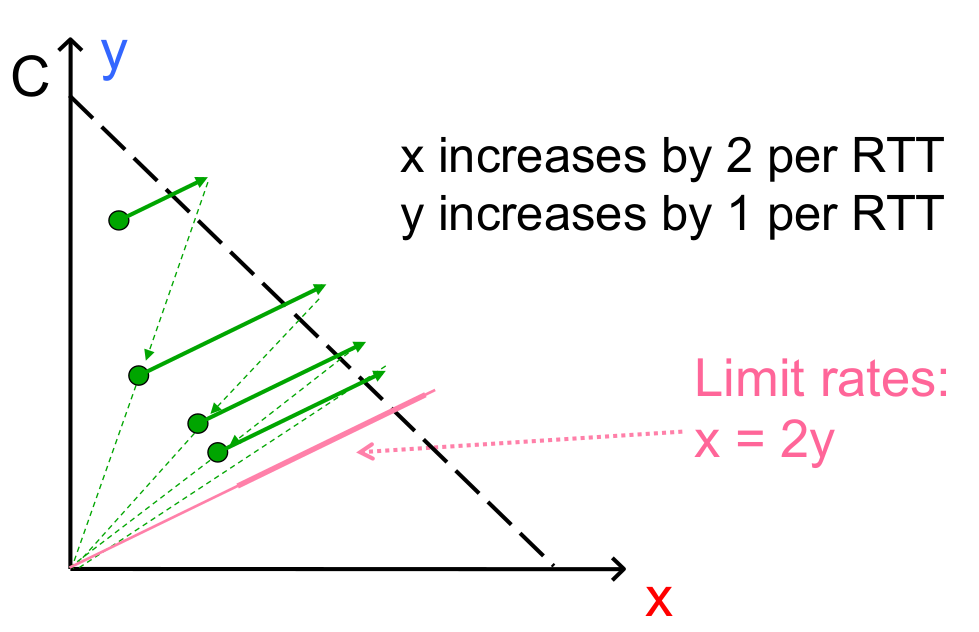
\includegraphics[width=\textwidth]{lazy/cwnd-faster.png}
\end{figure}
\subsubsection{Larger Initial Window}
\begin{figure}[H]
    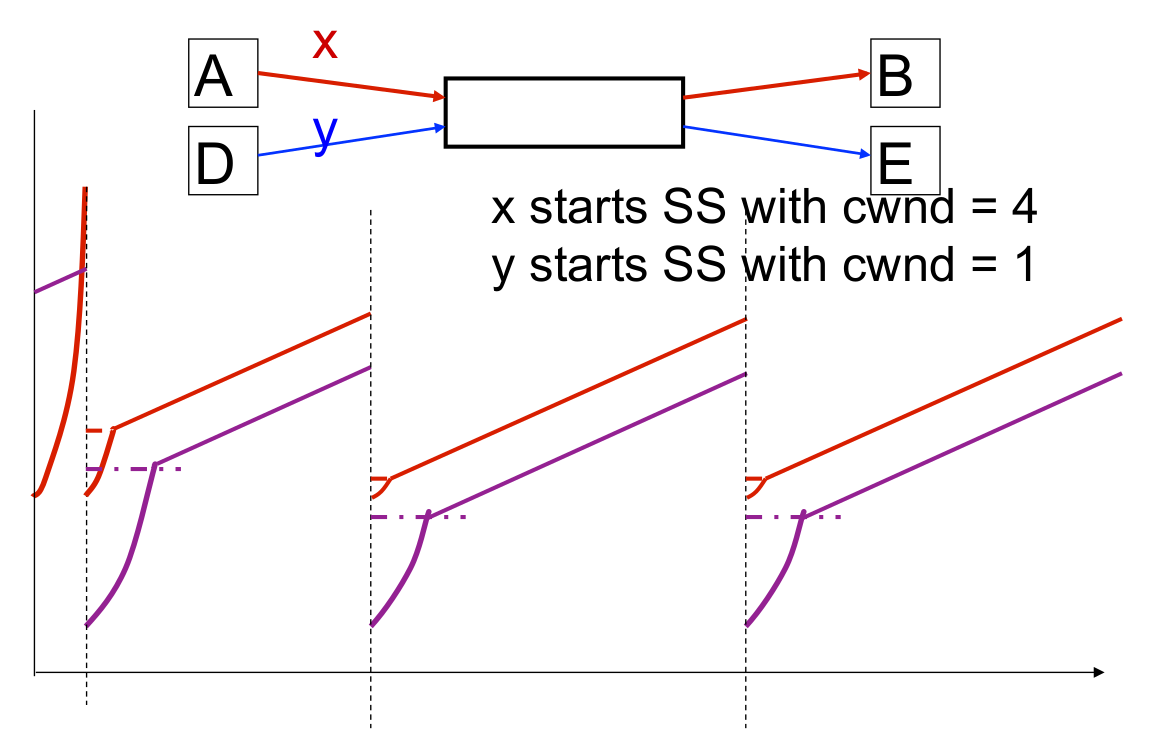
\includegraphics[width=\textwidth]{lazy/larger-initial-window.png}
\end{figure}
\subsubsection{Open Many Connections}
\begin{itemize}[nosep]
    \item Web Browser: has to download $k$ objects for a page
          \begin{itemize}[nosep]
              \item Open many connections or download sequentially?
                    \begin{figure}[H]
                        \centering
                        \tikzsetnextfilename{open-many-connections}
                        \begin{tikzpicture}
                            \node[draw,rectangle] (a) {$A$};
                            \node[draw,rectangle,below =of a] (d) {$D$};
                            \node[minimum width=3cm, minimum height=1cm,draw,rectangle,below right=-0.1cm and 1cm of a] (n) {};
                            \node[draw,rectangle,above right=0.1cm and 1cm of n] (b) {$B$};
                            \node[draw,rectangle,below=of b] (e) {$E$};

                            \draw[red, thick, ->] (a) -- (n) node[pos=0.5,above] {$x$};
                            \draw[red, thick, ->] (n) -- (b);
                            \draw[blue, thick, ->] (d) -- (n) node[pos=0.5,above] {$y$};;
                            \draw[blue, thick, ->] (n) -- (e);
                        \end{tikzpicture}
                    \end{figure}
              \item Assume:
                    \begin{itemize}[nosep]
                        \item $A$ opens 10 connections to $B$
                        \item $B$ opens 1 connection to $E$
                    \end{itemize}
              \item TCP is fair among connections
                    \begin{itemize}[nosep]
                        \item $A$ gets 10 times more bandwidth than $B$
                    \end{itemize}
          \end{itemize}
\end{itemize}
\subsubsection{Exploiting Implicit Assumptions}
\begin{itemize}[nosep]
    \item Savage, et al., CCR 1999
          \begin{itemize}[nosep]
              \item TCP Congestion Control with a Misbehaving Receiver
              \item \url{https://cseweb.ucsd.edu/~savage/papers/CCR99.pdf}
          \end{itemize}
    \item Exploits ambiguity of meaning of ACK
          \begin{itemize}[nosep]
              \item ACKs can specify any byte range for error control
              \item Congestion control assumes ACKs cover entire sent segments
          \end{itemize}
\end{itemize}
\subsubsection{ACK Division Attack}
\begin{itemize}[nosep]
    \item Receiver: \textit{``upon receiving a segment with $N$ bytes, divide the bytes into $M$ groups and ackowledge each group separately''}
    \item Sender will grow $M$ times faster
    \item Could cause growth to 4GB in 4 RTTs!
          \begin{itemize}[nosep]
              \item $M = N = 1460$
          \end{itemize}
\end{itemize}
\subsubsection{Defense}
\begin{itemize}[nosep]
    \item Appropriate Byte Counting
          \begin{itemize}[nosep]
              \item \phantom{}[RFC 3465 (2003), RFC 5681 (2009)]
              \item In slow start, $\texttt{cwnd} += \min(N, \texttt{MSS})$ where $N$ is the number of newly acknowledged bytes in the received ACK
          \end{itemize}
\end{itemize}
\subsubsection{DupACK Spoofing}
\begin{itemize}[nosep]
    \item Receiver: \textit{``Upon receiving a data segment, the receiver sends a long stream of acknowledgments for the last sequence number received''}
    \item Sender sends at a rate proportional to the ACK rate
\end{itemize}
\subsubsection{Optimistic ACKing}
\begin{itemize}[nosep]
    \item Receiver: \textit{``Upon receiving a data segment, the receiver sends a stream of acknowledgments anticipating data that will be sent by the sender''}
\end{itemize}
\subsubsection{Cheating TCP and Game Theory}
\begin{figure}[H]
    \centering
    \tikzsetnextfilename{cheating-tcp-and-game-theory}
    \begin{tikzpicture}
        \node[draw,rectangle] (a) {$A$};
        \node[draw,rectangle,below =of a] (d) {$D$};
        \node[minimum width=3cm, minimum height=1cm,draw,rectangle,below right=-0.1cm and 1cm of a] (n) {};
        \node[draw,rectangle,above right=0.1cm and 1cm of n] (b) {$B$};
        \node[draw,rectangle,below=of b] (e) {$E$};

        \draw[red, thick, ->] (a) -- (n) node[pos=0.5,above] {$x$};
        \draw[red, thick, ->] (n) -- (b);
        \draw[blue, thick, ->] (d) -- (n) node[pos=0.5,above] {$y$};;
        \draw[blue, thick, ->] (n) -- (e);

        \draw[thick] (0, -3) rectangle (6, -5);
        \draw (0, -3) rectangle (3, -4);
        \draw (0, -4) rectangle (3, -5);
        \draw (3, -3) rectangle (6, -4);
        \draw (3, -4) rectangle (6, -5);

        \node at (1.5, -3.3) {\textcolor{red}{22}, \textcolor{blue}{22}};
        \node at (4.5, -3.3) {\textcolor{red}{10}, \textcolor{blue}{35}};
        \node at (1.5, -4.3) {\textcolor{red}{35}, \textcolor{blue}{10}};
        \node at (4.5, -4.3) {\textcolor{red}{15}, \textcolor{blue}{15}};

        \node[red] at (-1.5, -3.5) {Increases by 1};
        \node[red] at (-1.5, -4.5) {Increases by 5};
        \node[red] at (-1.5, -2.5) {$A$};
        \draw[red,thick,->] (-1.5, -2.75) -- (-1.5, -3.25);

        \node[blue] at (1.5, -2.5) {Increases by 1};
        \node[blue] at (4.5, -2.5) {Increases by 5};
        \node[blue] at (-0.5, -2.5) {$D$};
        \draw[blue,thick,->] (-.25, -2.5) -- (0.25, -2.5);

        \node[align=left] at (8.5, -5) {Too aggressive\\$\to$Losses\\$\to$Throughput falls};
        \draw[->] (7,-4.5) -- (6,-4.5);

        \node at (0, -6) {\textcolor{teal}{Individual incentives:} cheating pays};
        \node at (0.7, -6.5) {\textcolor{teal}{Social incentives:} better off without cheating};
    \end{tikzpicture}
\end{figure}